% 物理理論レポート用テンプレート
\documentclass[11pt,a4paper]{ltjsarticle}

% パッケージの読み込み
\usepackage{luatexja}
\usepackage{luatexja-fontspec}
\usepackage[margin=25mm]{geometry}
\usepackage{amsmath,amssymb,amsthm}
\usepackage{mathtools}
\usepackage{physics}
\usepackage{siunitx}
\usepackage{tensor}
\usepackage{booktabs}
\usepackage{graphicx}
\usepackage{tikz}
\usepackage{tikz-feynman}
\usepackage{pgfplots}
\usepackage{tcolorbox}
\usepackage{xcolor}
\usepackage{fancyhdr}
\usepackage{url}
\usepackage{hyperref}

% フォント設定
\setmainfont{Noto Serif CJK JP}
\setsansfont{Noto Sans CJK JP}
\setmonofont{Noto Sans Mono CJK JP}

% 物理学用の定理環境
\theoremstyle{definition}
\newtheorem{definition}{定義}[section]
\newtheorem{law}{法則}[section]
\newtheorem{principle}{原理}[section]

\theoremstyle{plain}
\newtheorem{theorem}{定理}[section]
\newtheorem{lemma}[theorem]{補題}
\newtheorem{corollary}[theorem]{系}
\newtheorem{proposition}[theorem]{命題}

\theoremstyle{remark}
\newtheorem{remark}{注意}[section]
\newtheorem{example}{例}[section]
\newtheorem{application}{応用}[section]

% 証明環境の日本語化
\renewcommand{\proofname}{証明}

% 色の定義
\definecolor{accentblue}{RGB}{52,152,219}
\definecolor{accentgreen}{RGB}{46,204,113}
\definecolor{accentorange}{RGB}{230,126,34}
\definecolor{accentred}{RGB}{231,76,60}
\definecolor{accentpurple}{RGB}{155,89,182}

% tcolorboxのスタイル定義
\newtcolorbox{theorybox}[1][]{
    colback=accentblue!10,
    colframe=accentblue,
    fonttitle=\bfseries,
    title={重要な理論},
    #1
}

\newtcolorbox{equationbox}[1][]{
    colback=accentgreen!10,
    colframe=accentgreen,
    fonttitle=\bfseries,
    title={基礎方程式},
    #1
}

\newtcolorbox{physicalbox}[1][]{
    colback=accentorange!10,
    colframe=accentorange,
    fonttitle=\bfseries,
    title={物理的解釈},
    #1
}

\newtcolorbox{applicationbox}[1][]{
    colback=accentpurple!10,
    colframe=accentpurple,
    fonttitle=\bfseries,
    title={応用・発展},
    #1
}

% 物理記号のショートカット(hbarはphysicsパッケージで定義済み)
\newcommand{\kB}{k_{\text{B}}}
\newcommand{\NA}{N_{\text{A}}}

% ベクトル記法
\renewcommand{\vec}[1]{\boldsymbol{#1}}
\newcommand{\uvec}[1]{\hat{\boldsymbol{#1}}}

% 電磁気学用
\newcommand{\Efield}{\vec{E}}
\newcommand{\Bfield}{\vec{B}}
\newcommand{\Jfield}{\vec{J}}
\newcommand{\Hfield}{\vec{H}}
\newcommand{\Dfield}{\vec{D}}

% 量子力学用(physicsパッケージで多くが定義済み)
\renewcommand{\psi}{\Psi}
\newcommand{\Ham}{\hat{H}}

% 熱力学用
\newcommand{\entropy}{S}
\newcommand{\enthalpy}{H}
\newcommand{\gibbs}{G}
\newcommand{\helmholtz}{F}

% ヘッダー・フッター設定
\pagestyle{fancy}
\fancyhf{}
\fancyhead[L]{物理理論レポート}
\fancyhead[R]{\today}
\fancyfoot[C]{\thepage}

% ハイパーリンク設定
\hypersetup{
    colorlinks=true,
    linkcolor=accentblue,
    urlcolor=accentblue,
    citecolor=accentblue
}

% タイトル情報
\title{\Huge\textbf{物理理論:理論題目}}
\author{学籍番号:XXXXXXXX \\氏名:山田 太郎}
\date{\today}

\begin{document}

\maketitle

\tableofcontents
\clearpage

\section{はじめに}

物理学における〇〇理論は、自然界の基本的な現象を統一的に理解するための重要な枠組みである。本レポートでは、この理論の数学的定式化から物理的解釈、そして現代物理学への応用まで、包括的に考察する。

\begin{theorybox}
本レポートで扱う主要な理論的要素:
\begin{itemize}
    \item 基礎原理と公理系
    \item 数学的定式化
    \item 物理的解釈と意味
    \item 実験的検証と応用
\end{itemize}
\end{theorybox}

\section{理論的基礎}

\subsection{基本原理}

\begin{principle}[最小作用の原理]
\label{prin:least-action}
物理系の運動は、作用積分
\begin{equation}
    S = \int_{t_1}^{t_2} L(q_i, \dot{q}_i, t) \dd{t}
\end{equation}
を停留値にする軌道で記述される。ここで、$L$はラグランジアン、$q_i$は一般化座標である。
\end{principle}

この原理から、オイラー・ラグランジュ方程式が導出される:

\begin{equation}
    \frac{d}{dt}\pdv{L}{\dot{q}_i} - \pdv{L}{q_i} = 0
    \label{eq:euler-lagrange}
\end{equation}

\subsection{ハミルトン形式}

ルジャンドル変換により、ラグランジアン形式からハミルトニアン形式への移行が可能である:

\begin{align}
    p_i &= \pdv{L}{\dot{q}_i} \quad \text{(一般化運動量)} \\
    H(q_i, p_i, t) &= \sum_i p_i \dot{q}_i - L \quad \text{(ハミルトニアン)}
\end{align}

\begin{equationbox}
ハミルトンの正準方程式:
\begin{align}
    \dot{q}_i &= \pdv{H}{p_i} \\
    \dot{p}_i &= -\pdv{H}{q_i}
\end{align}
\end{equationbox}

\section{量子力学への拡張}

\subsection{正準量子化}

古典力学から量子力学への移行は、正準交換関係の導入により実現される:

\begin{equation}
    [\hat{q}_i, \hat{p}_j] = i\hbar\delta_{ij}
\end{equation}

\begin{theorem}[シュレーディンガー方程式]
量子系の時間発展は、以下の方程式で記述される:
\begin{equation}
    i\hbar\pdv{\psi}{t} = \Ham\psi
    \label{eq:schrodinger}
\end{equation}
ここで、$\psi$は波動関数、$\Ham$はハミルトン演算子である。
\end{theorem}

\subsection{調和振動子の解}

1次元調和振動子のハミルトニアンは:

\begin{equation}
    \Ham = \frac{\hat{p}^2}{2m} + \frac{1}{2}m\omega^2\hat{q}^2
\end{equation}

生成・消滅演算子を導入すると:

\begin{align}
    \hat{a} &= \sqrt{\frac{m\omega}{2\hbar}}(\hat{q} + \frac{i\hat{p}}{m\omega}) \\
    \hat{a}^\dagger &= \sqrt{\frac{m\omega}{2\hbar}}(\hat{q} - \frac{i\hat{p}}{m\omega})
\end{align}

\begin{physicalbox}
物理的解釈:
\begin{itemize}
    \item $\hat{a}^\dagger$:エネルギー量子を1つ生成
    \item $\hat{a}$:エネルギー量子を1つ消滅
    \item エネルギー固有値:$E_n = \hbar\omega(n + \frac{1}{2})$
    \item 零点エネルギー:$E_0 = \frac{1}{2}\hbar\omega$
\end{itemize}
\end{physicalbox}

\section{場の量子論への発展}

\subsection{Klein-Gordon方程式}

相対論的スカラー場の方程式:

\begin{equation}
    (\partial_\mu\partial^\mu + m^2c^2/\hbar^2)\phi = 0
\end{equation}

ここで、$\partial_\mu = (\frac{1}{c}\frac{\partial}{\partial t}, -\nabla)$である。

\subsection{Dirac方程式}

スピン1/2粒子(フェルミオン)の相対論的方程式:

\begin{equation}
    (i\gamma^\mu\partial_\mu - mc/\hbar)\psi = 0
\end{equation}

ガンマ行列$\gamma^\mu$は以下の反交換関係を満たす:

\begin{equation}
    \{\gamma^\mu, \gamma^\nu\} = 2g^{\mu\nu}I_4
\end{equation}

\begin{figure}[htbp]
    \centering
    \begin{tikzpicture}
        \begin{feynman}
            \vertex (a) at (-2,0);
            \vertex (b) at (0,0);
            \vertex (c) at (2,0);
            \vertex (d) at (0,1.5);
            \vertex (e) at (0,-1.5);
            
            \diagram* {
                (a) -- [fermion] (b) -- [fermion] (c),
                (b) -- [photon] (d),
                (b) -- [photon] (e),
            };
            
            \node at (-2,-0.3) {$e^-$};
            \node at (2,-0.3) {$e^-$};
            \node at (0.3,1.5) {$\gamma$};
            \node at (0.3,-1.5) {$\gamma$};
        \end{feynman}
    \end{tikzpicture}
    \caption{電子-光子相互作用のファインマン図}
    \label{fig:feynman}
\end{figure}

\section{電磁気学との統合}

\subsection{マクスウェル方程式}

電磁場の基礎方程式:

\begin{align}
    \nabla \cdot \Efield &= \frac{\rho}{\varepsilon_0} \\
    \nabla \cdot \Bfield &= 0 \\
    \nabla \times \Efield &= -\pdv{\Bfield}{t} \\
    \nabla \times \Bfield &= \mu_0\Jfield + \mu_0\varepsilon_0\pdv{\Efield}{t}
\end{align}

\subsection{ゲージ理論}

電磁場はベクトルポテンシャル$A^\mu = (\phi/c, \vec{A})$で記述される:

\begin{align}
    \Efield &= -\nabla\phi - \pdv{\vec{A}}{t} \\
    \Bfield &= \nabla \times \vec{A}
\end{align}

ゲージ変換不変性:

\begin{align}
    \phi' &= \phi - \pdv{\Lambda}{t} \\
    \vec{A}' &= \vec{A} + \nabla\Lambda
\end{align}

\begin{applicationbox}
ゲージ理論の応用:
\begin{itemize}
    \item 電弱統一理論(ワインバーグ・サラム理論)
    \item 量子色力学(QCD)
    \item 標準模型における対称性の自発的破れ
\end{itemize}
\end{applicationbox}

\section{熱力学・統計力学との関連}

\subsection{統計力学の基礎}

分配関数による統計的記述:

\begin{equation}
    Z = \sum_i e^{-\beta E_i} = \tr(e^{-\beta\Ham})
\end{equation}

ここで、$\beta = 1/\kB T$である。

熱力学量との関係:

\begin{align}
    F &= -\kB T \ln Z \quad \text{(自由エネルギー)} \\
    \langle E \rangle &= -\pdv{\ln Z}{\beta} \quad \text{(内部エネルギー)} \\
    \entropy &= \kB(\ln Z + \beta\langle E \rangle) \quad \text{(エントロピー)}
\end{align}

\subsection{量子統計}

\begin{table}[htbp]
    \centering
    \caption{量子統計の比較}
    \label{tab:quantum-statistics}
    \begin{tabular}{lcc}
        \toprule
        統計 & 分布関数 & 適用粒子 \\
        \midrule
        Fermi-Dirac & $f_{FD} = \frac{1}{e^{\beta(E-\mu)} + 1}$ & フェルミオン \\
        Bose-Einstein & $f_{BE} = \frac{1}{e^{\beta(E-\mu)} - 1}$ & ボソン \\
        Maxwell-Boltzmann & $f_{MB} = e^{-\beta(E-\mu)}$ & 古典粒子 \\
        \bottomrule
    \end{tabular}
\end{table}

\section{現代物理学への応用}

\subsection{標準模型}

素粒子物理学の標準模型は、以下の対称性群に基づく:

\begin{equation}
    SU(3)_C \times SU(2)_L \times U(1)_Y
\end{equation}

\begin{itemize}
    \item $SU(3)_C$:強い相互作用(量子色力学)
    \item $SU(2)_L \times U(1)_Y$:電弱統一理論
\end{itemize}

\subsection{一般相対性理論}

アインシュタイン方程式:

\begin{equation}
    G_{\mu\nu} = \frac{8\pi G}{c^4}T_{\mu\nu}
\end{equation}

ここで、$G_{\mu\nu}$はアインシュタインテンソル、$T_{\mu\nu}$はエネルギー運動量テンソルである。

\begin{figure}[htbp]
    \centering
    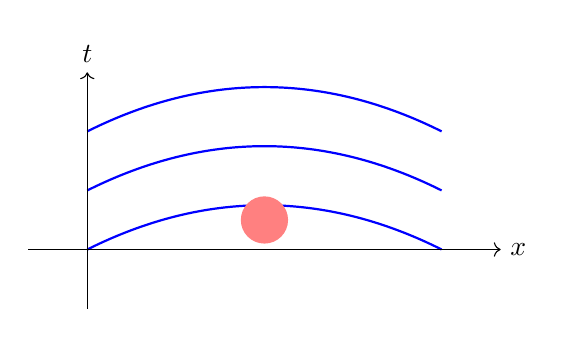
\begin{tikzpicture}[scale=1.5]
        % 時空の曲がりを表現
        \draw[thick, blue] (0,0) .. controls (1,0.5) and (2,0.5) .. (3,0);
        \draw[thick, blue] (0,0.5) .. controls (1,1) and (2,1) .. (3,0.5);
        \draw[thick, blue] (0,1) .. controls (1,1.5) and (2,1.5) .. (3,1);
        
        % 質量による時空の歪み
        \fill[red!50] (1.5,0.25) circle (0.2);
        \node at (1.5,-0.2) {質量};
        
        % 座標軸
        \draw[->] (-0.5,0) -- (3.5,0) node[right] {$x$};
        \draw[->] (0,-0.5) -- (0,1.5) node[above] {$t$};
        
        \node at (1.5,1.8) {時空の曲がり};
    \end{tikzpicture}
    \caption{質量による時空の曲がりの概念図}
    \label{fig:spacetime}
\end{figure}

\section{数値計算例}

\subsection{調和振動子の固有値}

量子調和振動子の最低3つのエネルギー準位:

\begin{align}
    E_0 &= \frac{1}{2}\hbar\omega = \SI{0.5}{\hbar\omega} \\
    E_1 &= \frac{3}{2}\hbar\omega = \SI{1.5}{\hbar\omega} \\
    E_2 &= \frac{5}{2}\hbar\omega = \SI{2.5}{\hbar\omega}
\end{align}

\begin{figure}[htbp]
    \centering
    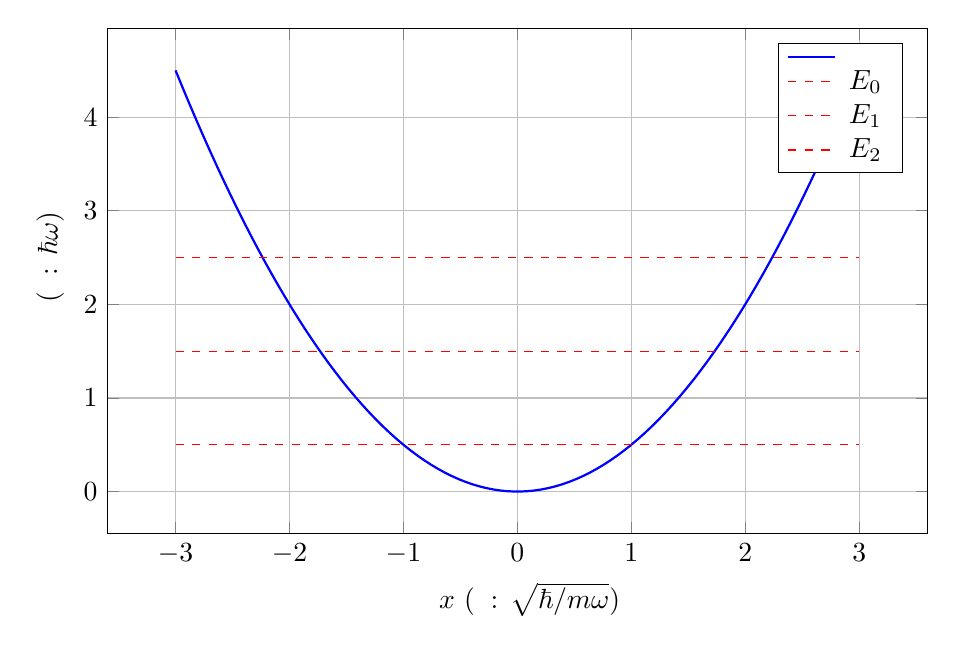
\begin{tikzpicture}
        \begin{axis}[
            xlabel={位置 $x$ (単位: $\sqrt{\hbar/m\omega}$)},
            ylabel={エネルギー (単位: $\hbar\omega$)},
            grid=major,
            legend pos=north east,
            width=12cm,
            height=8cm,
            domain=-3:3,
            samples=100
        ]
        \addplot[blue, thick] {0.5*x^2};
        \addplot[red, dashed] coordinates {(-3,0.5) (3,0.5)};
        \addplot[red, dashed] coordinates {(-3,1.5) (3,1.5)};
        \addplot[red, dashed] coordinates {(-3,2.5) (3,2.5)};
        \legend{ポテンシャル, $E_0$, $E_1$, $E_2$}
        \end{axis}
    \end{tikzpicture}
    \caption{調和振動子のエネルギー準位}
    \label{fig:harmonic-levels}
\end{figure}

\section{考察と発展}

\subsection{理論の統一性}

本レポートで考察した理論群は、物理学の統一的理解に向けた重要なステップを示している:

\begin{enumerate}
    \item 古典力学から量子力学への発展
    \item 特殊相対性理論と量子力学の融合(場の量子論)
    \item 四つの基本相互作用の統一理論への挑戦
\end{enumerate}

\subsection{今後の課題}

\begin{applicationbox}[title={未解決問題と発展方向}]
\begin{itemize}
    \item 量子重力理論(超弦理論、ループ量子重力)
    \item 暗黒物質・暗黒エネルギーの正体
    \item 量子もつれと量子情報理論
    \item 多体量子系の非平衡統計力学
\end{itemize}
\end{applicationbox}

\section{まとめ}

本レポートでは、物理学の基礎理論から現代的な発展まで、包括的に考察した。主な結論は以下の通りである:

\begin{enumerate}
    \item 最小作用の原理は、古典力学から場の理論まで統一的な枠組みを提供する
    \item 対称性と保存則の関係(ネーターの定理)は、物理法則の深い構造を明らかにする
    \item 量子力学と相対性理論の融合は、素粒子物理学と宇宙論の発展を可能にした
    \item 統計力学は、微視的理論と巨視的現象を結ぶ重要な架け橋である
\end{enumerate}

これらの理論的枠組みは、現代物理学の基盤として今後の研究発展に不可欠な役割を果たし続けるであろう。

\begin{thebibliography}{99}
\bibitem{landau1} L. D. Landau, E. M. Lifshitz, \textit{Mechanics}, 3rd Edition, Butterworth-Heinemann, 1976.
\bibitem{landau2} L. D. Landau, E. M. Lifshitz, \textit{Quantum Mechanics: Non-Relativistic Theory}, 3rd Edition, Pergamon Press, 1977.
\bibitem{sakurai} J. J. Sakurai, J. Napolitano, \textit{Modern Quantum Mechanics}, 2nd Edition, Addison-Wesley, 2010.
\bibitem{peskin} M. E. Peskin, D. V. Schroeder, \textit{An Introduction to Quantum Field Theory}, Westview Press, 1995.
\bibitem{weinberg} S. Weinberg, \textit{The Quantum Theory of Fields}, Cambridge University Press, 1995.
\bibitem{japanese1} 江沢洋, 『量子力学I』, 裳華房, 2002.
\bibitem{japanese2} 田中正, 『統計力学』, 岩波書店, 1988.
\bibitem{japanese3} 中西襄, 『場の量子論』, 培風館, 1987.
\end{thebibliography}

\end{document}